\documentclass[11pt,a4paper]{article}
\usepackage[utf8]{inputenc}
\usepackage[margin=2.5cm]{geometry}
\usepackage{graphicx}
\usepackage{float}
\usepackage{xcolor}
\usepackage{listings}
\lstset{escapeinside={<@}{@>}}
\usepackage{hyperref}

\graphicspath{ {./images/} }

\title{DNS laboratory - Group 2}
\author{Carlo Ramponi, Luca De Menego, Matteo Zanotto}
\date{04 May 2022}

\definecolor{codegreen}{rgb}{0,0.6,0}
\definecolor{codegray}{rgb}{0.5,0.5,0.5}
\definecolor{codepurple}{rgb}{0.58,0,0.82}
\definecolor{backcolour}{rgb}{0.95,0.95,0.92}

\lstdefinestyle{mystyle}{
    backgroundcolor=\color{backcolour},   
    commentstyle=\color{codegreen},
    keywordstyle=\color{magenta},
    numberstyle=\tiny\color{codegray},
    stringstyle=\color{codepurple},
    basicstyle=\ttfamily\footnotesize,
    breakatwhitespace=false,         
    breaklines=true,                 
    captionpos=b,                    
    keepspaces=true,                 
    numbers=left,                    
    numbersep=5pt,                  
    showspaces=false,                
    showstringspaces=false,
    showtabs=false,                  
    tabsize=2
}

\lstset{style=mystyle}

\begin{document}
\begin{titlepage}

\centering
    \vfill
    \vskip3cm
    \Large Department of Information Engineering and Computer Science
    \vskip0.5cm
    \Large (DISI)
    \vskip2cm
    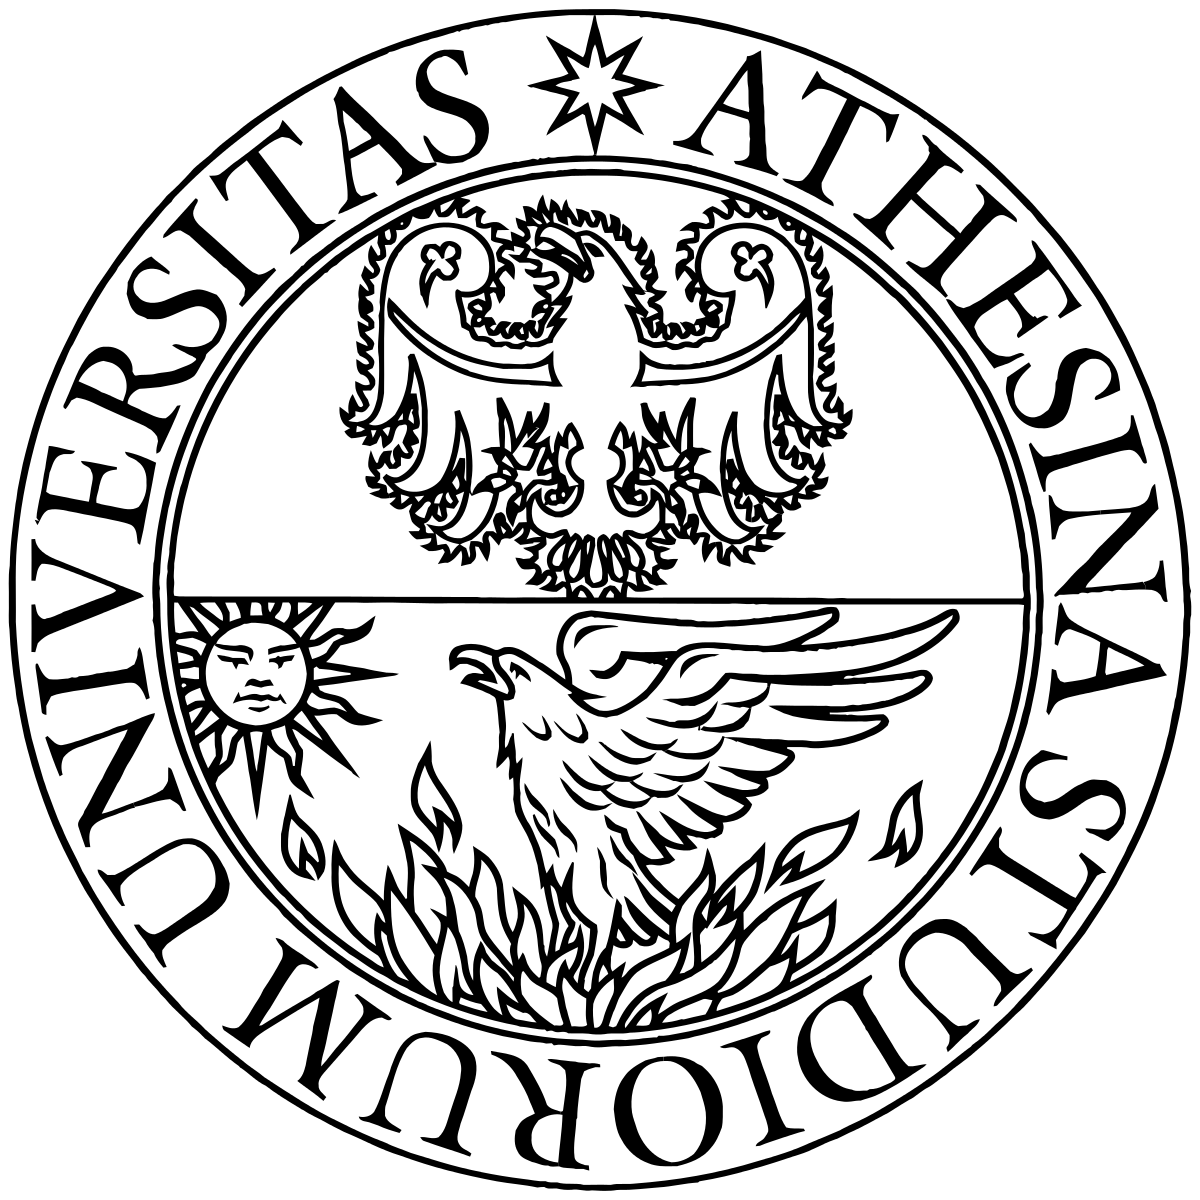
\includegraphics[width=8cm]{logo_unitn.png}
    \vskip2cm
    \textbf{\Large Network Security - A.Y. 2021/2022}
    \vskip2cm
    \textbf{\LARGE DNS}
    \vskip0.2cm
    \textbf{\LARGE Cache poisoning and Kaminsky attack}
    \vskip4cm
    \Large Carlo Ramponi, Luca De Menego, Matteo Zanotto
    \vfill

\end{titlepage}

\clearpage

\tableofcontents

\clearpage

\section{DNS specification}

\subsection{What is the DNS}

The \emph{Domain Name System} is an essential Internet service that maps human-readable hostnames to IP addresses that machines in networking can use.

\noindent
The DNS was developed to provide a consistent namespace for referring to internet resources such as host domain names or mailboxes. It defines standard formats for representing the resource data and methods to query the database.

\hfill \break
\noindent
The DNS was developed with scalability in mind to adapt to the increasing sheer size of internet data and usage: it is implemented in a distributed hierarchical manner as a tree structure, where
more fine-grained information about the resources is accessed by walking down a delegation mechanism.

\noindent
Additionally, local caching is applied to improve the performance: already known information is stored so it can be served directly without repeating queries.

\subsection{Typical DNS messages flow}
DNS queries typically follow a redirect flow between various name servers along the hierarchy
until the resource is resolved. This is because each name server either answers the question
posed in the query or refers the requester to another set of name servers when it cannot
resolve the query.

\hfill \break
\noindent
In a typical name resolution scenario, the client will generate a DNS query on the browser
when trying to connect to a domain. A DNS recursive resolver will handle the query.

\noindent
The recursive resolver will traverse the DNS hierarchy to resolve
the domain if caches are empty. Starting from a root name, it will be redirected to an appropriate top-level domain
name server for the input address, which will redirect to an authoritative name server, that can directly resolve the question without further recursion.

\noindent
The recursive resolver returns the address to the client, which can finally connect to the
domain.

\hfill \break
\noindent
A query ID, generated by the resolver and required to have the same value for both question and answer, identifies each interaction between the recursive resolver and the other name servers. This lightweight authentication mechanism allows a
recursive resolver to know that it is receiving a reply from a name server about the
question it has sent. Responses that do not match the query ID will be discarded by the resolver,
while legitimate responses are stored in the cache.

\subsection{DNS messages format}

A DNS packet is structured as a message with a header containing a set of permanently present fixed
fields and four sections of data content.

\noindent
The header fields contain the 16-bit query ID, a set of flags (for example, for signaling if the message is a question or an answer or for error handling), and a set of numbers for quantifying
the entities in the data section.

\noindent
The data section differs depending on if it is a question or an answer. However, it is generally structured
in four sections: question data, answer data, authority data, and additional data. A question
message will be composed of a question data section with the name, type, and class of the
resource that needs to be resolved. In contrast, an answer message will contain different data in the
answer section depending on the returned resource type. For example, in the case of a
domain name resolution, it will contain the A-type domain name with the associated IP address. In contrast, the redirection to another name server will contain an NS-type answer with the name of the
name server and an A-type answer for the name server's address.

\hfill \break
\noindent
A DNS message is typically carried over a UDP packet for the fast performance requirements
of the service.

\subsection{Resources representation}
All DNS data is stored in a core data structure called Resource Record (RR), which is internally
composed of a series of fields and is identified by a name.

\hfill \break
\noindent
The fields of resource record are:
\begin{itemize}
\item Type, which specifies the abstract type of the resource in this resource record. The most common types are \texttt{A} for domain addresses, \texttt{NS} for name servers of a domain, \texttt{SOA} for authority information, and \texttt{MX} for mail exchanges.
\item Class, for the protocol that it refers to, almost always with value \texttt{IN} for the Internet.
\item Data, for type and class depending on data of the Resource Record. For example, in the case of an A-type resource record, it will be an IP address, while for an NS resource record, it will be a domain name.
\item TTL, the time to live of the information on the cache
\end{itemize}

\section{DNS implementation: Bind}

During this laboratory, we will practically interact with a DNS implementation using \textit{Bind}, one of the most widely-used DNS server implementations on the Internet. It is an open-source program currently
maintained by the Internet Software Consortium, offering a complete
implementation of the DNS protocol, and in particular, it can be used to set up an authoritative
name server, a recursive resolver, or a forwarder.

\subsection{Bind configuration}

With Bind, the DNS server configuration happens through the \texttt{named.conf} file (usually located
in the \texttt{/etc/bind} directory) in which it is possible to specify the options applied to the Bind server and
the domains zones for which the server holds authoritative data.

\noindent
In particular, when configuring a Bind server, there are many possible options. Some initial
basic steps include:
\begin{itemize}
\item the definition of a list of trusted clients from which to accept queries with the \texttt{allow-query}
option, for example, by specifying only from internal network IP addresses.
\item the definition with the \texttt{forwards} option of a custom list of other DNS server addresses to
forward queries.
\item the specification of the cache file location with \texttt{dump-file}. 
\end{itemize}
These are just the basics of running a DNS server, but there are a lot of more advanced
options that can be configured with Bind, such as multi-threading, mechanisms for zone transfers
between masters and slaves and detailed logging.

\noindent
Additionally, both as an excellent system hardening practice and for network resources usage, the
The bind DNS server should be executed on a dedicated machine.

\noindent
A configuration step must also be performed on clients' machines that will connect to the Bind
DNS server: the \texttt{resolve.conf} file must be modified to change the default DNS address to
which queries will be sent with the address of the Bind name server.

\subsection{Zone files}

Managing an authoritative name server with Bind means defining the domain zone files in
which resource records are stored. Usually, the zone definitions happen on external files included in the main \texttt{named.conf} file in the \texttt{zone} blocks.

\noindent
Bind follows the DNS specification for the syntax of the zone files very closely, to the point
where even the Bind documentation often overlaps with the RFC 1034 when describing the zone
part of the configuration. In particular, Bind uses a textual format for expressing Resource Records consisting of entries of name, data, type, class, and time to live fields.

\noindent
At the beginning of each zone definition, there is usually a Start Of Authority resource record
that reports critical data about the zone, such as the administrator or the caching and refreshing
time configurations.

\noindent
Bind also supports some directives in the zone files to simplify its syntax. For example, the \texttt{@} sign will refer to the zone name defined when importing the file in \texttt{named.conf}, or the \texttt{\$TTL} variable for expressing a global value for the time to live of entries (but will be overwritten when further specified).

\section{Laboratory introduction}

\subsection{Katharà}
To experiment with the DNS implementation, we will use a tool called Katharà, which is an open
source container-based network emulation system that allows to setup network environments
for testing or developing purposes.

\noindent
Katharà works by emulating specific network devices starting from a Docker image containing network-oriented software such as routing daemons (RIP, OSPF, etc.), an HTTP server, firewall
utilities, and diagnostic tools (ping, tcpdump, dig). Also, it comes with a Bind distribution.
By configuring the appropriate software, it is possible to emulate almost any kind of network
scenario.

\subsection{Laboratory network topology}

With Katharà, we have created a simulated network that we will use to demonstrate the attacks.
It has the following topology:
\begin{itemize}
\item a victim sub-network, in which there is a victim host and a recursive forwarder DNS
resolver, to which the victim sends queries when resolving domain names.
\item a domain sub-network for the ‘example.com‘ organization, composed of two web
servers that form the foo.example.com and bar.example.com domains and an authoritative
name server for resolving the addresses in the domain.
\item the attacker sub-network, composed of the attacker device from which attacks are
performed, a malicious web server, and a malicious name server.
\item an external network to which all the gateway routers of the subnetworks are connected so
they can communicate with each other through statically defined routes. This network also
contains a top-level domain name server for .com domains, to which the victim resolver
will direct queries for any unknown domain.
\end{itemize}

\begin{figure}[h!]
  \centering
  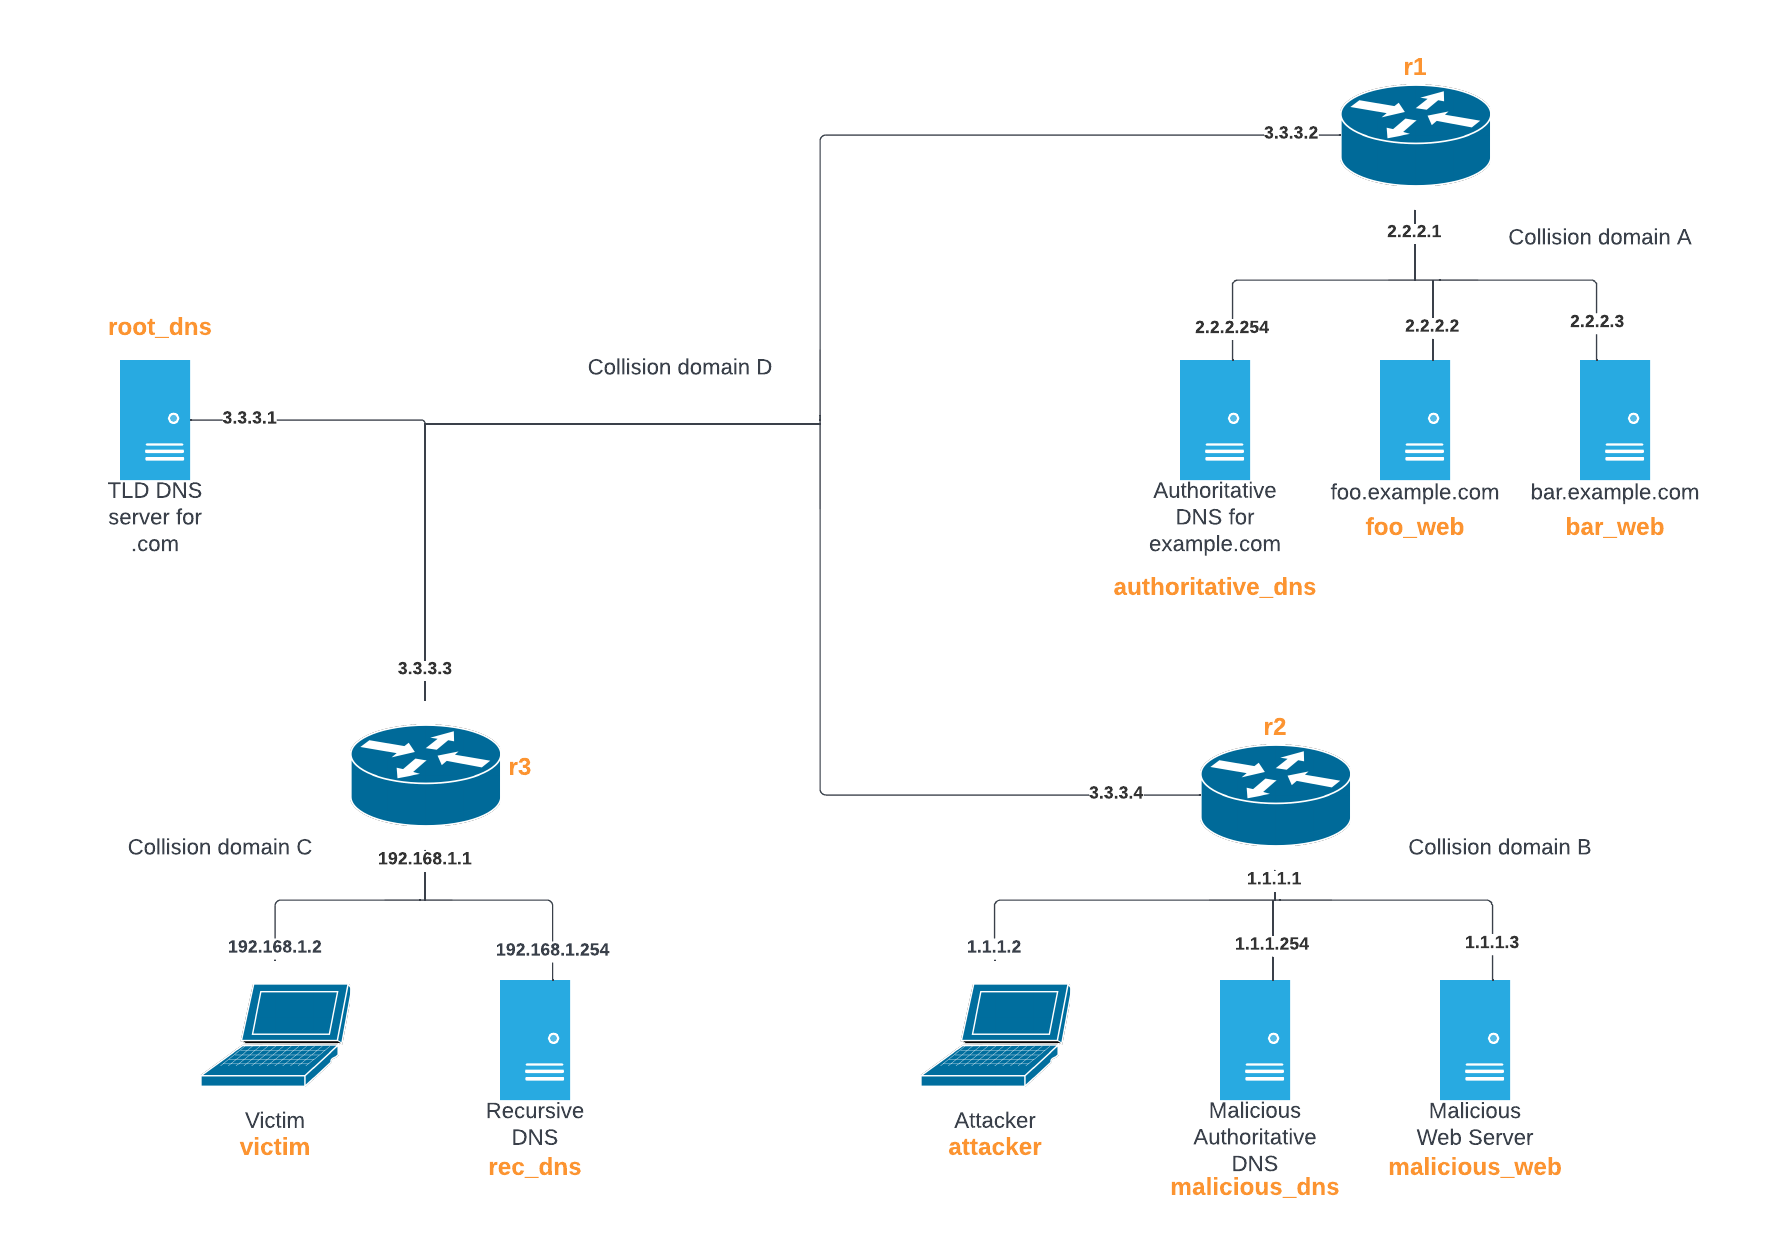
\includegraphics[width=\textwidth]{network-topology.png}
  \caption{Laboratory network topology}
\end{figure}

\section{DNS Cache Poisoning}

\subsection{Attack introduction}
This first exercise will focus on a DNS Cache Poisoning attack. The main idea is
to inject wrong information into a recursive nameserver’s cache. In our case, in particular, we
will try to map the domain \texttt{foo.example.com} to the attacker’s
malicious website inside the target DNS cache.
\\
\\
\noindent
In order to perform such an attack, it is obviously not enough to send random DNS responses
with the chosen \texttt{A} record: the DNS will only accept \textbf{valid} responses \textbf{to pending queries}. The most important fields our fake response will need to match are:
\begin{itemize}
    \item the source port: the chosen UDP source port for the communication between two entities;
    \item the query ID: a unique identifier assigned when the query was created;
    \item the query section: every response must contain a copy of the original request.
\end{itemize}

\subsection{The attack in details}
\label{subsec:attack-details}

\begin{figure}[h]
    \centering
    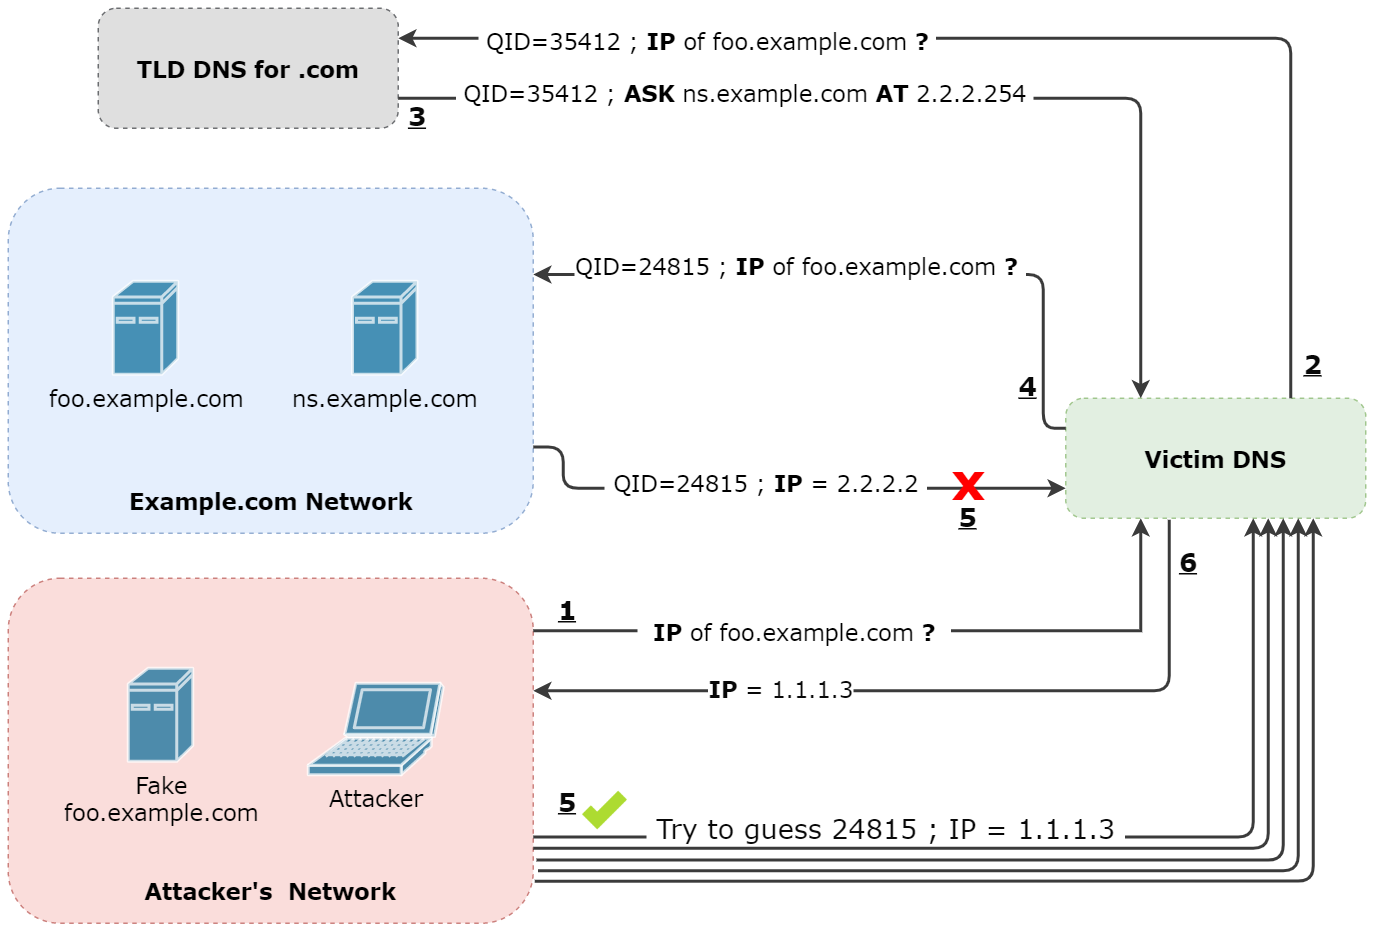
\includegraphics[width=\textwidth]{cache-poisoning-attack.png}
    \caption{Cache Poisoning Attack scheme}
    \label{fig:cache-poisoning-attack}
\end{figure}

\noindent
Before diving into the implementation, it is crucial to understand how the attack will be performed. Following Figure \ref{fig:cache-poisoning-attack}, the attack can be represented with six steps:
\begin{enumerate}
    \item the attacker asks the victim recursive nameserver what the \texttt{A} record for\\\texttt{foo.example.com} is;
    \item the recursive nameserver, since it does not know the answer, asks it to the Top Level Domain nameserver for \texttt{.com};
    \item the TLD nameserver answers with: 
    \begin{itemize}
        \item an NS record stating that the authoritative nameserver for the requested domain is \texttt{ns.example.com};
        \item an A record mapping \texttt{ns.example.com} to its IP address \texttt{2.2.2.254}.
    \end{itemize}
    \item now the recursive DNS can ask, for the last time, what is the A record for \texttt{foo.example.com} to the authoritative nameserver;
    \item a \textbf{race condition} takes place:
    \begin{itemize}
        \item the authoritative nameserver replies with the correct A record, containing \texttt{2.2.2.2};
        \item the attacker tries to guess the transaction ID of the last query, sending fake responses stating that \texttt{foo.example.com} is at \texttt{1.1.1.3}, a malicious web server controlled by the attacker.
    \end{itemize}
    \item finally, the recursive nameserver will answer the attacker with the \texttt{A} record it got first.
\end{enumerate}

\noindent
At the end of this process, if the attacker is able to correctly guess the query ID and send the fake response before the real authoritative nameserver, the attack succeeds. Notice that an important assumption was made, since we decided to fix the source port, to simulate the original attack. Hence in our environment, source ports are not randomized. In Section \ref{sec:final-considerations}, additional information can be found about this.



\subsection{Sniff a legitimate communication}
The explained flow can be easily sniffed and analyzed with essential command-line tools. Let us try to reconstruct it from a legitimate DNS query.
\\
\\
\noindent
First of all, open one terminal, connect to the recursive DNS and start listening to UDP packets:
\begin{lstlisting}
 <@\textcolor{codegray}{:>}@> kathara lstart  <@\textcolor{codegreen}{\# Start the laboratory if you haven't already}@>
 <@\textcolor{codegray}{:>}@> kathara connect rec_dns <@\textcolor{codegreen}{\# Connect to the recursive DNS}@>
 <@\textcolor{codegray}{rec-dns :>}@> tcpdump -vv udp port 53    <@\textcolor{codegreen}{\# Start listening to all udp packets}@>
\end{lstlisting}
\noindent
\\
Now open another terminal, connect to the victim and gather DNS information on\\\texttt{hi.example.com} using the \texttt{dig} utility:
\begin{lstlisting}
 <@\textcolor{codegray}{:>}@> kathara connect victim <@\textcolor{codegreen}{\# Connect to the victim's machine}@>
 <@\textcolor{codegray}{victim :>}@> dig hi.example.com    <@\textcolor{codegreen}{\# Gather DNS information on hi.example.com}@>
\end{lstlisting}
\noindent
\\
The result of \texttt{tcpdump} is shown in Figure \ref{fig:tcpdump-res}. The flow is clearly the same as the one explained in Subsection \ref{subsec:attack-details}, without the attacker's manipulation involved. It is important to note that the query IDs are always respected between requests and replies, and here the final response of the authoritative server contains the correct \texttt{A} record.
\\
\\
\noindent
One only thing is still missing: the response from the recursive nameserver to the client. This is available in the \texttt{dig}'s response, visible in Figure \ref{fig:dig-res}. Apart from the sections' results, that at this point should be clear, the same Query ID of the first \texttt{tcpdump}'s request output should be seen.

\begin{figure}[h]
    \centering
    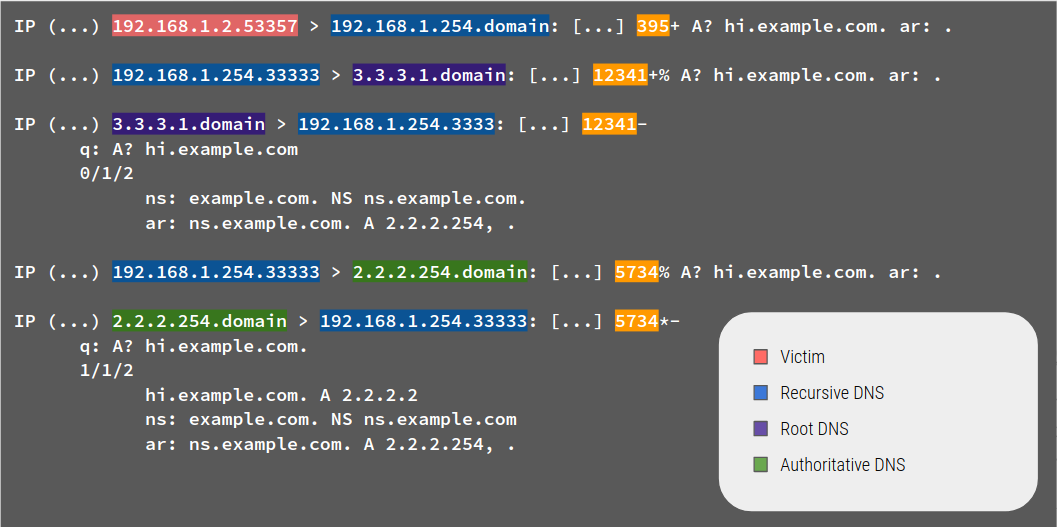
\includegraphics[width=\textwidth]{tcpdump-res.png}
    \caption{tcpdump's result}
    \label{fig:tcpdump-res}
\end{figure}

\begin{figure}[h]
    \centering
    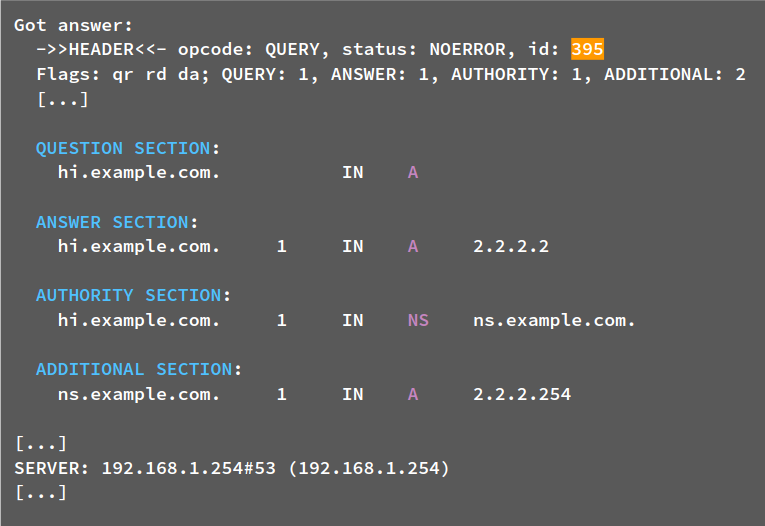
\includegraphics[width=\textwidth]{dig-result.png}
    \caption{dig's result}
    \label{fig:dig-res}
\end{figure}

\subsection{The Workspace}

Inside the lab directory, you will find a \textbf{shared folder}, common to all Kathará
machines. All updates performed to the files inside this folder will be immediately visible
to everyone. This means that you can:
\begin{itemize}
    \item work on the scripts inside it from the host machine, with the editor of your choice;
    \item when you are ready, connect to the attacker's machine with \texttt{kathara connect attacker};
    \item compile the script with \texttt{g++ -o script-name /shared/script-name.cpp -ltins};
    \item run it with \texttt{./script-name}
\end{itemize}

\noindent
All the scripts are written in C++, and for packet crafting the \texttt{libtins}
library has been used, which provides an easy-to-use and efficient platform for
manipulating network packets.

\subsection{Implementation of the attack}
The cache poisoning implementation is available inside the \texttt{cache-poisoning.cpp}
file, in the script folder. Following the flow explained in subsection
\ref{subsec:attack-details}, in the first part a DNS query is created. In particular,
as shown in Figure \ref{fig:cache-poisoning-first}:
\begin{itemize}
    \item the type of the request is set to \texttt{DNS::QUERY};
    \item the query ID can be any number we want since we are creating the query ourselves;
    \item the recursion is allowed, so the recursive DNS will recursively ask the same query to upper-level nameservers;
    \item the actual query will be for the \texttt{A} record of \texttt{foo.example.com};
    \item the final packet is constructed, composed of three parts: IP, UDP, and DNS.
\end{itemize}

\begin{figure}[h]
    \centering
    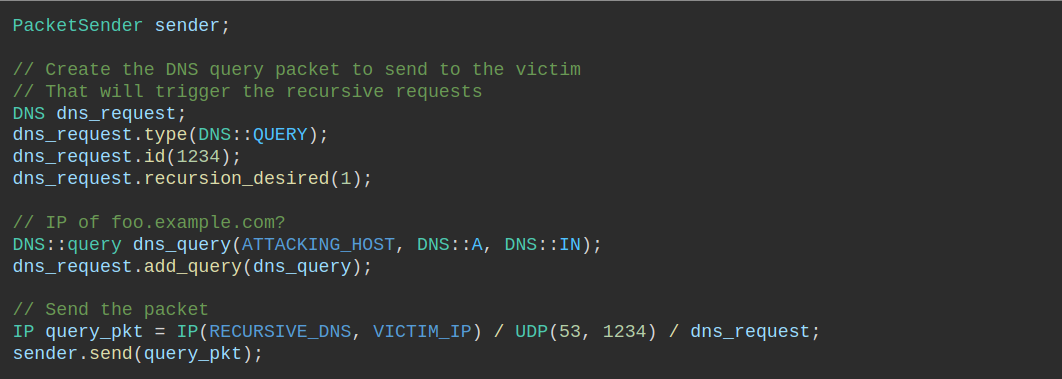
\includegraphics[width=\textwidth]{cache-poisoning-first.png}
    \caption{First part of the cache poisoning script: generate a DNS query}
    \label{fig:cache-poisoning-first}
\end{figure}

\noindent
In the second part of the script available in Figure \ref{fig:cache-poisoning-second},
instead, we will try to guess the Query ID, sending fake packets containing the
malicious A record. Here the main steps are the following:

\begin{itemize}
    \item loop through every possible Query ID, creating a packet for each one of them;
    \item set the type of the DNS packet to \texttt{DNS::RESPONSE};
    \item set the current Query ID of the loop;
    \item allow the recursion, for the same reason as before;
    \item add the original query into the packet, as any DNS response without the corresponding query will be simply dropped by a DNS server.
\end{itemize}

\noindent
To finalize the script, we need to complete the DNS answer and initialize the IP packet correctly:
\begin{enumerate}
    \item \textbf{DNS answer creation}: what we want to achieve is a DNS \texttt{A} record stating that the domain \texttt{foo.example.com} should resolve to \texttt{1.1.1.3}. So the first parameter must be set to \texttt{ATTACKING\_DOMAIN}, and the second to \texttt{MALICIOUS\_WEBSERVER};
    \item \textbf{IP packet completion}: we want to send this fake response to the recursive DNS, pretending to be the legitimate authoritative nameserver it contacted. Since the first parameter represents the destination and the second one the source, we should put respectively \texttt{RECURSIVE\_DNS} and \texttt{AUTHORITATIVE\_DNS}.
\end{enumerate}

\begin{figure}[h]
    \centering
    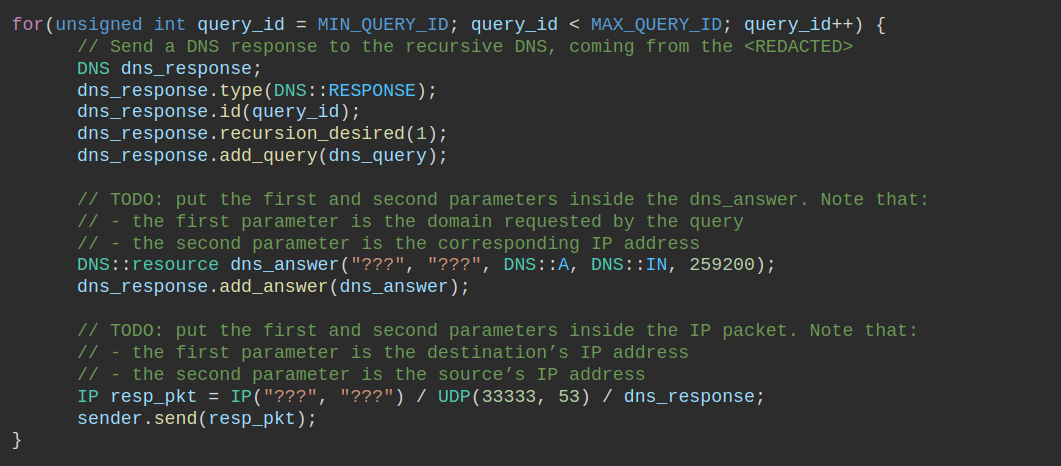
\includegraphics[width=\textwidth]{cache-poisoning-second.png}
    \caption{Second part of the cache poisoning script: try to guess the Query ID and poison the cache of the target DNS}
    \label{fig:cache-poisoning-second}
\end{figure}

\newpage
\subsection{Final Steps}
\noindent
Before compiling and running the attack, however, there is one important step missing. We want to be sure to win the race condition against the real authoritative DNS. That's why we will cheat a little bit, by adding a delay to it:
\begin{lstlisting}
 <@\textcolor{codegray}{:>}@> kathara connect authoritative_dns  <@\textcolor{codegreen}{\# Connect to the authoritative DNS}@>
 <@\textcolor{codegray}{authoritative-dns :>}@> tc qdisc add dev eth0 root netem delay 1500ms    <@\textcolor{codegreen}{\# Add delay}@>
\end{lstlisting}
\noindent
Now that the probability of success has increased a lot, we can compile and run the attack:
\begin{lstlisting}
 <@\textcolor{codegray}{:>}@> kathara connect attacker  <@\textcolor{codegreen}{\# Connect to the attacker's machine}@>
 <@\textcolor{codegray}{attacker :>}@> g++ -o cache-poisoning /shared/cache-poisoning.cpp -ltins    <@\textcolor{codegreen}{\# Compile}@>
 <@\textcolor{codegray}{attacker :>}@> ./cache-poisoning    <@\textcolor{codegreen}{\# Run}@>
\end{lstlisting}

\noindent
Since we are guessing the Query ID, the probability of success is not 100\%.
To verify whether the attack was successful or not there are two main ways:
\begin{enumerate}
    \item check the cache of the recursive DNS. You should see an A record for \texttt{foo.example.com} mapped to \texttt{1.1.1.3}.
    \begin{lstlisting}
     <@\textcolor{codegray}{:>}@> kathara connect rec_dns  <@\textcolor{codegreen}{\# Connect to the recursive DNS}@>
     <@\textcolor{codegray}{dns :>}@> rndc dumpdb -cache && grep "example.com" /var/cache/bind/dump.db     
     
     [...]
     foo.<@\textcolor{red}{example.com}@>.  259172  A   1.1.1.3
     [...]\end{lstlisting}
     \item check the effect on the victim's side by using \textit{links}, a simple console browser:
     \begin{lstlisting}
     <@\textcolor{codegray}{:>}@> kathara connect victim  <@\textcolor{codegreen}{\# Connect to the victim's machine}@>
     <@\textcolor{codegray}{victim :>}@> links    <@\textcolor{codegreen}{\# Launch the browser}@>\end{lstlisting}
     Type \textbf{'g'} and search \texttt{'http://foo.example.com'}. You should be redirected to the attacker's website, as can be seen in Figure \ref{fig:attacker-website}.
\end{enumerate}

\noindent
If in your case it didn't work, keep retrying: after some trials you should be able to guess the correct Query ID. You can even try to play with the delay: incrementing it would mean increasing your probability of success.

\begin{figure}[h!]
    \centering
    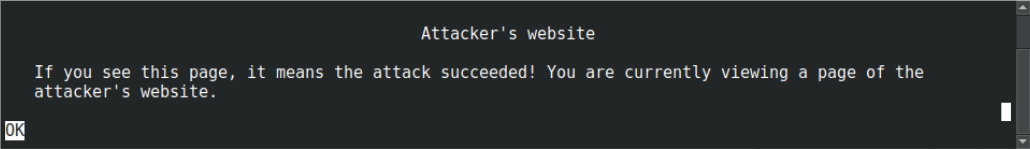
\includegraphics[width=\textwidth]{attacker-website.png}
    \caption{The attacker's website, visible after a correct execution of the cache poisoning attack}
    \label{fig:attacker-website}
\end{figure}

\newpage
\section{Kaminsky Attack}

\subsection{Attack introduction}

In the previous attack, we have successfully poisoned an \textbf{A} record in the
cache of the \emph{recursive DNS}, meaning that we gained full control over the
host \texttt{foo.example.com}.
\\
\\
\noindent
The \emph{Kaminsky attack} is a variant of the \emph{cache poisoning attack}, in
which we want to gain control over a full domain, instead of a single host, by
poisoning an \textbf{NS} record in the cache of the \emph{recursive DNS}.
\\
\\
\noindent
In our case, we want to gain control over \texttt{example.com}, so that all the
subdomains of \texttt{example.com} will be poisoned.

\subsection{The attack in details}

\begin{figure}[h!]
  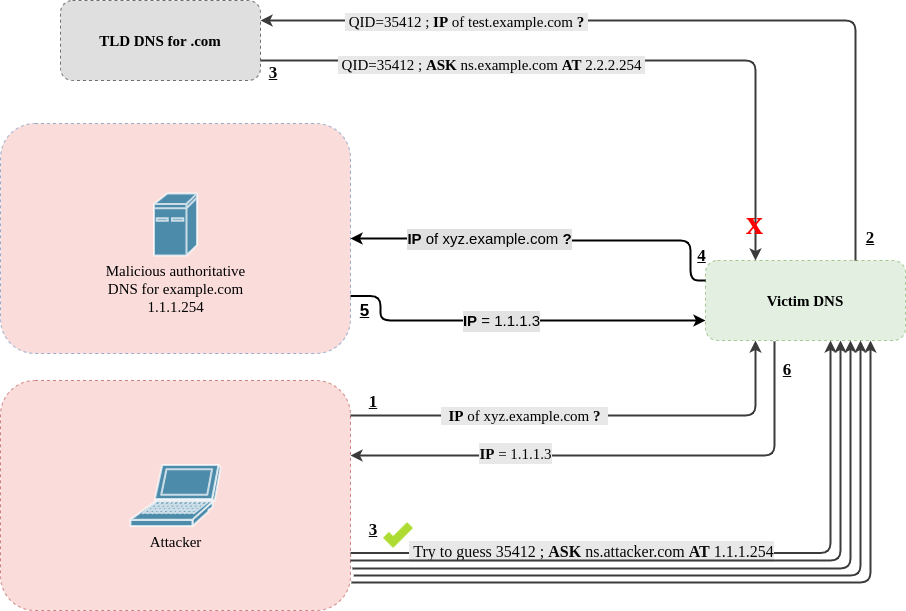
\includegraphics[width=\textwidth]{kaminsky-attack.png}
  \caption{Kaminsky Attack scheme}
  \label{fig:kaminsky-attack}
\end{figure}

\noindent
Here are the steps of this attack:
\begin{enumerate}
  \item the attacker asks the victim recursive DNS to resolve a random subdomain of
        \texttt{example.com} (e.g. \texttt{xyz.example.com}), so that it will probably
        not be already in his cache.
  \item the recursive DNS, since it doesn't know the domain, will ask the TLD domain the
        the same question.
  \item now a \textbf{race condition} takes place:
        \begin{itemize}
          \item the TLD will reply saying that \texttt{*.example.com} can be resolved
                by \texttt{ns.example.com} at \texttt{2.2.2.254}, which in the DNS language
                would be \texttt{FOR example.com ASK ns.example.com AT 2.2.2.254}.
          \item the attacker will try to guess the \textbf{Query ID} and send a poisoned response
                saying: \texttt{FOR example.com ASK ns.attacker.com AT 1.1.1.254}.
        \end{itemize}
  \item the recursive DNS will then ask the Authoritative DNS (whether it is the real
        one or the attacker's one) the same question,
  \item which will reply with an \textbf{A} record for \texttt{xyz.example.com},
  \item then the reply will be forwarded to the host that asked for it.
\end{enumerate}

\noindent
Also in this case, if the attacker can win the race condition, guessing the right
\textbf{Query ID} before the legitimate response from the TLD DNS arrives, then the attack
is successful.
\\
\\
\noindent
You can notice that the process is very similar to the previous attack, but this one
is way more powerful: it can poison a whole domain, not just a single host.

\subsection{The workspace}

Also, the workspace is very similar to the previous attack. There is a template of the
attack inside the lab's \textbf{shared} folder, which has to be completed. You can
compile and run the scripts in the same way.
\\
\\
\noindent
Let's first clean our environment, to make sure we start from a fresh installation of
the lab, by restarting all the containers:

\begin{lstlisting}
<@\textcolor{codegray}{:>}@> kathara lclean  <@\textcolor{codegreen}{\# Stop the lab and remove the containers}@>
<@\textcolor{codegray}{:>}@> kathara lstart  <@\textcolor{codegreen}{\# Restart the lab from scratch}@>
\end{lstlisting}

\noindent
\\
Once again we need to cheat a little bit, setting a delay on the server we want to beat
during the \textbf{race condition}, which in this case is the \emph{Top Level Domain}.

\begin{lstlisting}
<@\textcolor{codegray}{:>}@> kathara connect root_dns                       <@\textcolor{codegreen}{\# Connect to the TLD machine}@>
<@\textcolor{codegray}{root\_server :>}@> tc qdisc add dev eth0 root netem delay 1500ms   <@\textcolor{codegreen}{\# Set the delay}@>
\end{lstlisting}

\subsection{Implementation of the attack}

The first part of the attack, apart from the random choice of the subdomain, is the same
as the \emph{Cache Poisoning Attack}. So let's jump to the second part.

\begin{figure}[h!]
  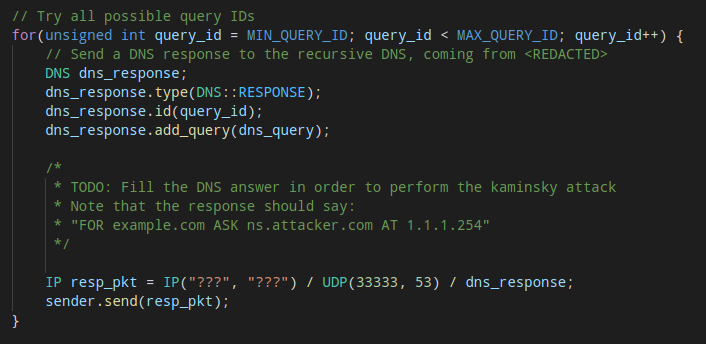
\includegraphics[width=\textwidth]{kaminsky-template.png}
  \caption{Kaminsky Attack template}
  \label{fig:kaminsky-attack-template}
\end{figure}

\noindent
\\
As we can see in figure \ref{fig:kaminsky-attack-template}, the malicious response has to be
built, like in the previous case, with:
\begin{itemize}
  \item \texttt{DNS::RESPONSE} as type,
  \item with the chosen \texttt{Query ID},
  \item and it has to include the original query.
\end{itemize}

\noindent
Now we need to complete this template by adding the Authoritative answer:
\begin{itemize}
  \item we need to include the \textbf{NS} entry for the \texttt{example.com} domain,
        which is the part: \texttt{"FOR example.com ASK ns.attacker.com"}
  \item and include the address of the give nameserver as an additional record, which is
        the part: \texttt{"AT 1.1.1.254"}
  \item and finally, complete the source and destination IP address, which are, respectively,
        the \texttt{TLD DNS} and the \texttt{recursive DNS}.
\end{itemize}

\begin{figure}[h!]
  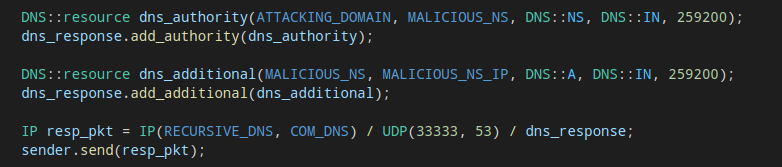
\includegraphics[width=\textwidth]{kaminsky-solution.png}
  \caption{Kaminsky Attack solution}
  \label{fig:kaminsky-attack-solution}
\end{figure}

\subsection{Run the attack}

Compile and run the scripts as usual:
\begin{lstlisting}
<@\textcolor{codegray}{:>}@> kathara connect attacker  <@\textcolor{codegreen}{\# Connect to the attacker's machine}@>
<@\textcolor{codegray}{attacker :>}@> g++ -o kaminsky /shared/kaminsky.cpp -ltins    <@\textcolor{codegreen}{\# Compile}@>
<@\textcolor{codegray}{attacker :>}@> ./kaminsky    <@\textcolor{codegreen}{\# Run}@>
\end{lstlisting}

\noindent
\\
Check if the attack was successful either by:
\begin{itemize}
  \item resolving any domain under \texttt{example.com}, from the victim machine
\begin{lstlisting}
<@\textcolor{codegray}{:>}@> kathara connect victim
<@\textcolor{codegray}{victim:/\#}@> dig foo.example.com
[...]
;; ANSWER SECTION:
<@\textcolor{codepurple}{foo.example.com.}@>        59815   IN      A       <@\textcolor{codepurple}{1.1.1.3}@>
[...]

<@\textcolor{codegray}{victim:/\#}@> dig bar.example.com
[...]
;; ANSWER SECTION:
<@\textcolor{codepurple}{bar.example.com.}@>        60000   IN      A       <@\textcolor{codepurple}{1.1.1.3}@>
[...]  
\end{lstlisting}
  \item or looking at the \emph{recursive DNS}'s cache.
\begin{lstlisting}
<@\textcolor{codegray}{:>}@> kathara connect rec_dns
<@\textcolor{codegray}{rec\_dns:/\#}@> rndc dumpdb -cache && grep "example.com" /var/cache/bind/dump.db
<@\textcolor{codepurple}{example.com.}@>            59921   NS      <@\textcolor{codepurple}{ns.attacker.com.}@>
<@\textcolor{codepurple}{uadrd.example.com.}@>       59919   A       <@\textcolor{codepurple}{1.1.1.3}@>
\end{lstlisting}
\end{itemize}

\noindent
Also in this case, if the attack didn't work, try to run the attack multiple times
or, if you have a slow computer, try to increase the \texttt{delay} in the
\emph{TLD DNS}'s machine.

\subsection{\texttt{\textcolor{codepurple}{dig}}ging into the attack}

Let's look at the packets that were sent during the attack.
\\
\\
\noindent
Clear the cache of the \emph{recursive DNS} and start capturing the traffic,
writing the output to a file in the \textbf{shared} folder,
so that it is accessible by the host machine:

\begin{lstlisting}
<@\textcolor{codegray}{:>}@> kathara connect rec_dns
<@\textcolor{codegray}{rec\_dns:/\#}@> rndc flush
<@\textcolor{codegray}{rec\_dns:/\#}@> tcpdump -i eth0 udp port 53 -w /shared/capture.pcap
\end{lstlisting}

\noindent
\\
Start the attack again from the \emph{attacker} machine:
\begin{lstlisting}
<@\textcolor{codegray}{:>}@> kathara connect attacker
<@\textcolor{codegray}{attacker :>}@> ./kaminsky
\end{lstlisting}

\noindent
\\
Wait a couple of seconds and stop the capture, now we can open the file with \emph{Wireshark}
and analyze it:

\begin{itemize}
  \item In figure \ref*{fig:wireshark-1} we can see the request made by the
        \emph{recursive DNS} (\texttt{192.168.1.254}) to the \emph{TLD DNS}
        (3.3.3.1).\\
        Wireshark also suggests to us which packet contains the response for
        this query (\textbf{59895}).
  \item In figure \ref{fig:wireshark-2} we can see, among all the malicious responses,
        the one that matched the right query ID (\textbf{0xe9f3}).
  \item Finally, in figure \ref{fig:wireshark-3} we see the legitimate response, sent by
        the \emph{TLD DNS}, which is marked as a \textbf{retransmission} since a reply
        for the query ID has already arrived (the malicious one).
\end{itemize}

\begin{figure}[h!]
  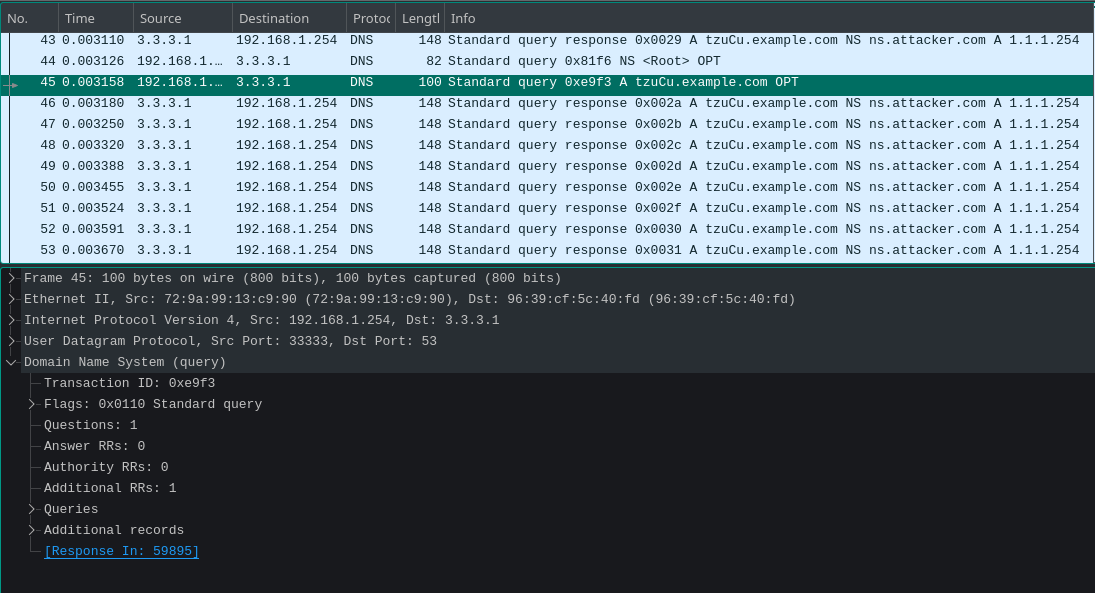
\includegraphics[width=\linewidth]{wireshark-1.png}
  \caption{The DNS query made by the \emph{recursive DNS} to the \emph{TLD DNS}}
  \label{fig:wireshark-1}
\end{figure}

\begin{figure}[h!]
  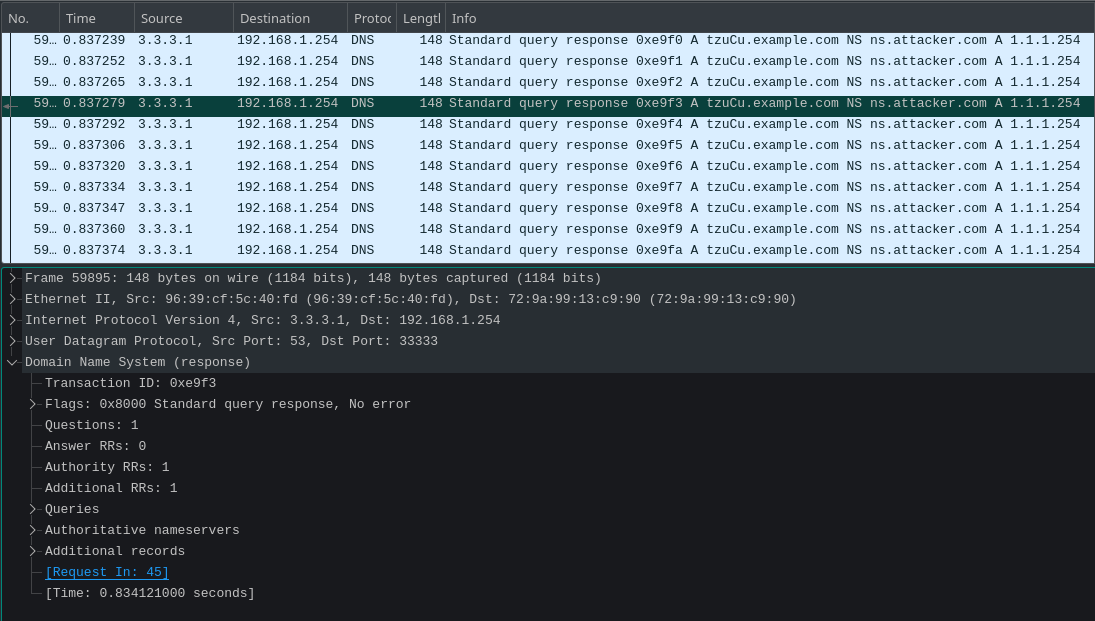
\includegraphics[width=\linewidth]{wireshark-2.png}
  \caption{The malicious response that matched the query ID}
  \label{fig:wireshark-2}
\end{figure}

\begin{figure}[h!]
  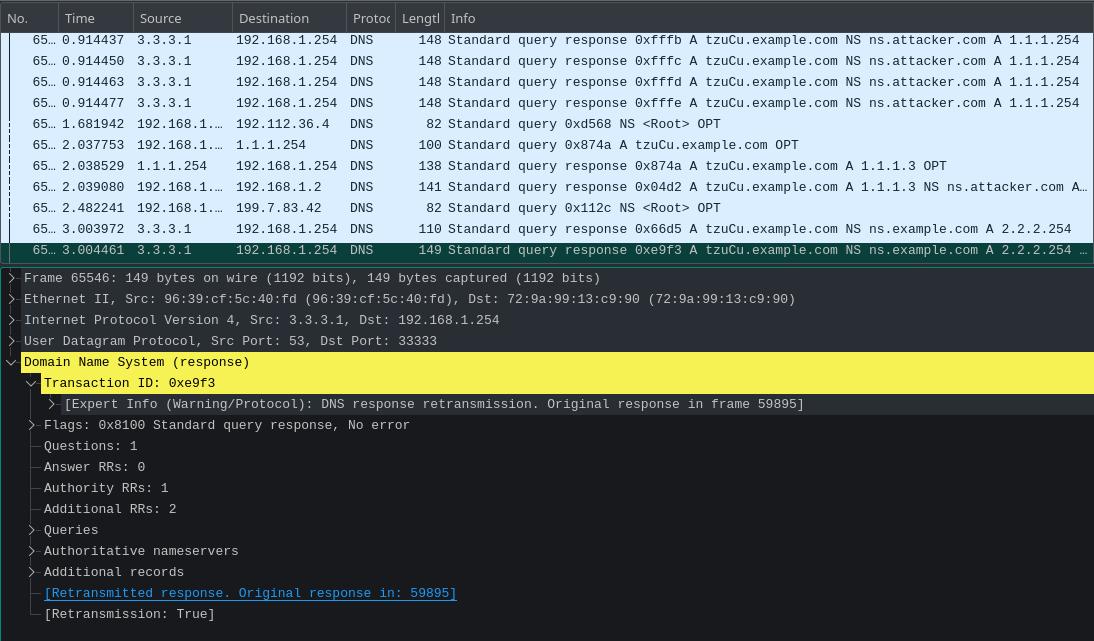
\includegraphics[width=\linewidth]{wireshark-3.png}
  \caption{The legitimate response}
  \label{fig:wireshark-3}
\end{figure}

\clearpage

\section{Final considerations}
\label{sec:final-considerations}

\subsection{Performing the attack nowadays}

Performing the attack nowadays is much harder than it was in early implementations of DNS servers. 

\noindent
As we have seen, the attacks are possible because of the small space of the query ID,
consisting of just 16 bits. Some early versions of DNS servers applied weak random algorithms
or even sequential procedures for the generation of this number, which made it easy for
attackers to predict the next query ID.

\noindent
This problem is mitigated by the use of pseudo-random number generators and the inclusion
of the source port, which is also randomized. In this way, since there are two 16 bits numbers
to guess, it is much harder to complete an attack in the narrow window of time while the victim
is going through the name resolution process. More specifically, considering $2^{16}$ bits for
the query ID times $2^{16}$ (excluding the reserved ports) bits for the source port we get
roughly 4 billion possible values to guess.

\subsection{DNSSEC}

Another counter measure is DNSSEC, that was developed to add data integrity and origin
authentication to DNS query replies, so that users can verify that the answers received
are indeed originated from the intended DNS server and have not been altered. In particular,
DNSSEC applies public-key cryptography to prove the authenticity of data with signatures,
by storing the public key in a new type of resource record and allowing resolvers to verify
the responses. DNSSEC creates a Public Key Infrastructure leveraging the already existing
DNS hierarchy so that each parent zone verifies the keys of its children zones.

\hfill \break
\noindent
However, DNSSEC deployment proved to be especially problematic. Scalability issues were
introduced by sustaining the PKI on the DNS hierarchy, as key changes require notifications
to the parent or child zones: for large TLD name servers this becomes infeasible due to the
high number of child zones. Moreover, the chain of authentication of the PKI infrastructure
holds for a certain name server only if all its parent nodes from the root name server have
also deployed DNSSEC; in reality, the PKI remains incomplete with isolated zones of DNSSEC
deployments.

\noindent
Other issues arose with the heavy usage of caching throughout DNS, such as changes in zones
keys not being immediately visible due to long TTLs (preventing resolvers to verify the data),
the management of keys rollover (periodical changes of the keys) and handling of exposed keys.

\hfill \break
\noindent
As of today, DNSSEC is still at an early level of deployment as it requires a conjunctive
effort by registrars, name servers administrators and network operators. Currently it is
estimated that only 30\% of DNS data is validated (as reported by the APNIC, the internet
registry of Pacific Asia).

\end{document}